\section{Résultats}
\begin{figure}[H]
  \centering
  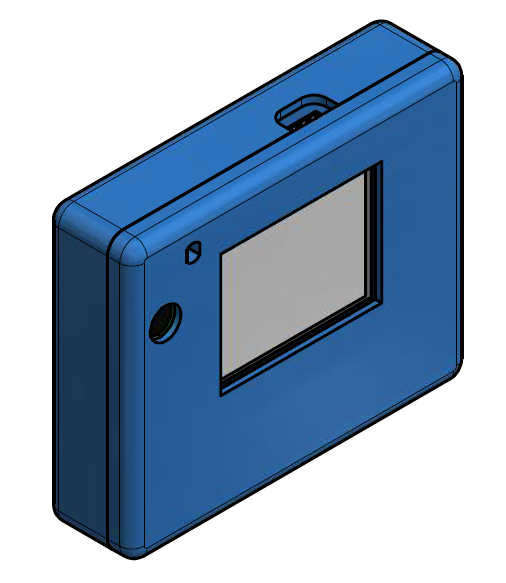
\includegraphics[width=0.5\linewidth]{mechanical/fullCase}
  \caption{Boîtier complet du PongBoy}
  \label{mech_pongboy}
\end{figure}
Le cahier des charges est respecté. La jouabilité est correcte.
Par manque de temps, et manque de ressources humaines,
les fonctionnalités comme le haut-parleur, et le mode multi-joueur n'ont pas
pu être implémentés.
\newpage

\section{Test}
De nombreux tests ont été réalisés pour vérifier la qualité du produit.
Ces tests ont permis de détecter de nombreux problèmes, qui ont bien
entendu été corrigés.
\begin{figure}[H]
  \centering
  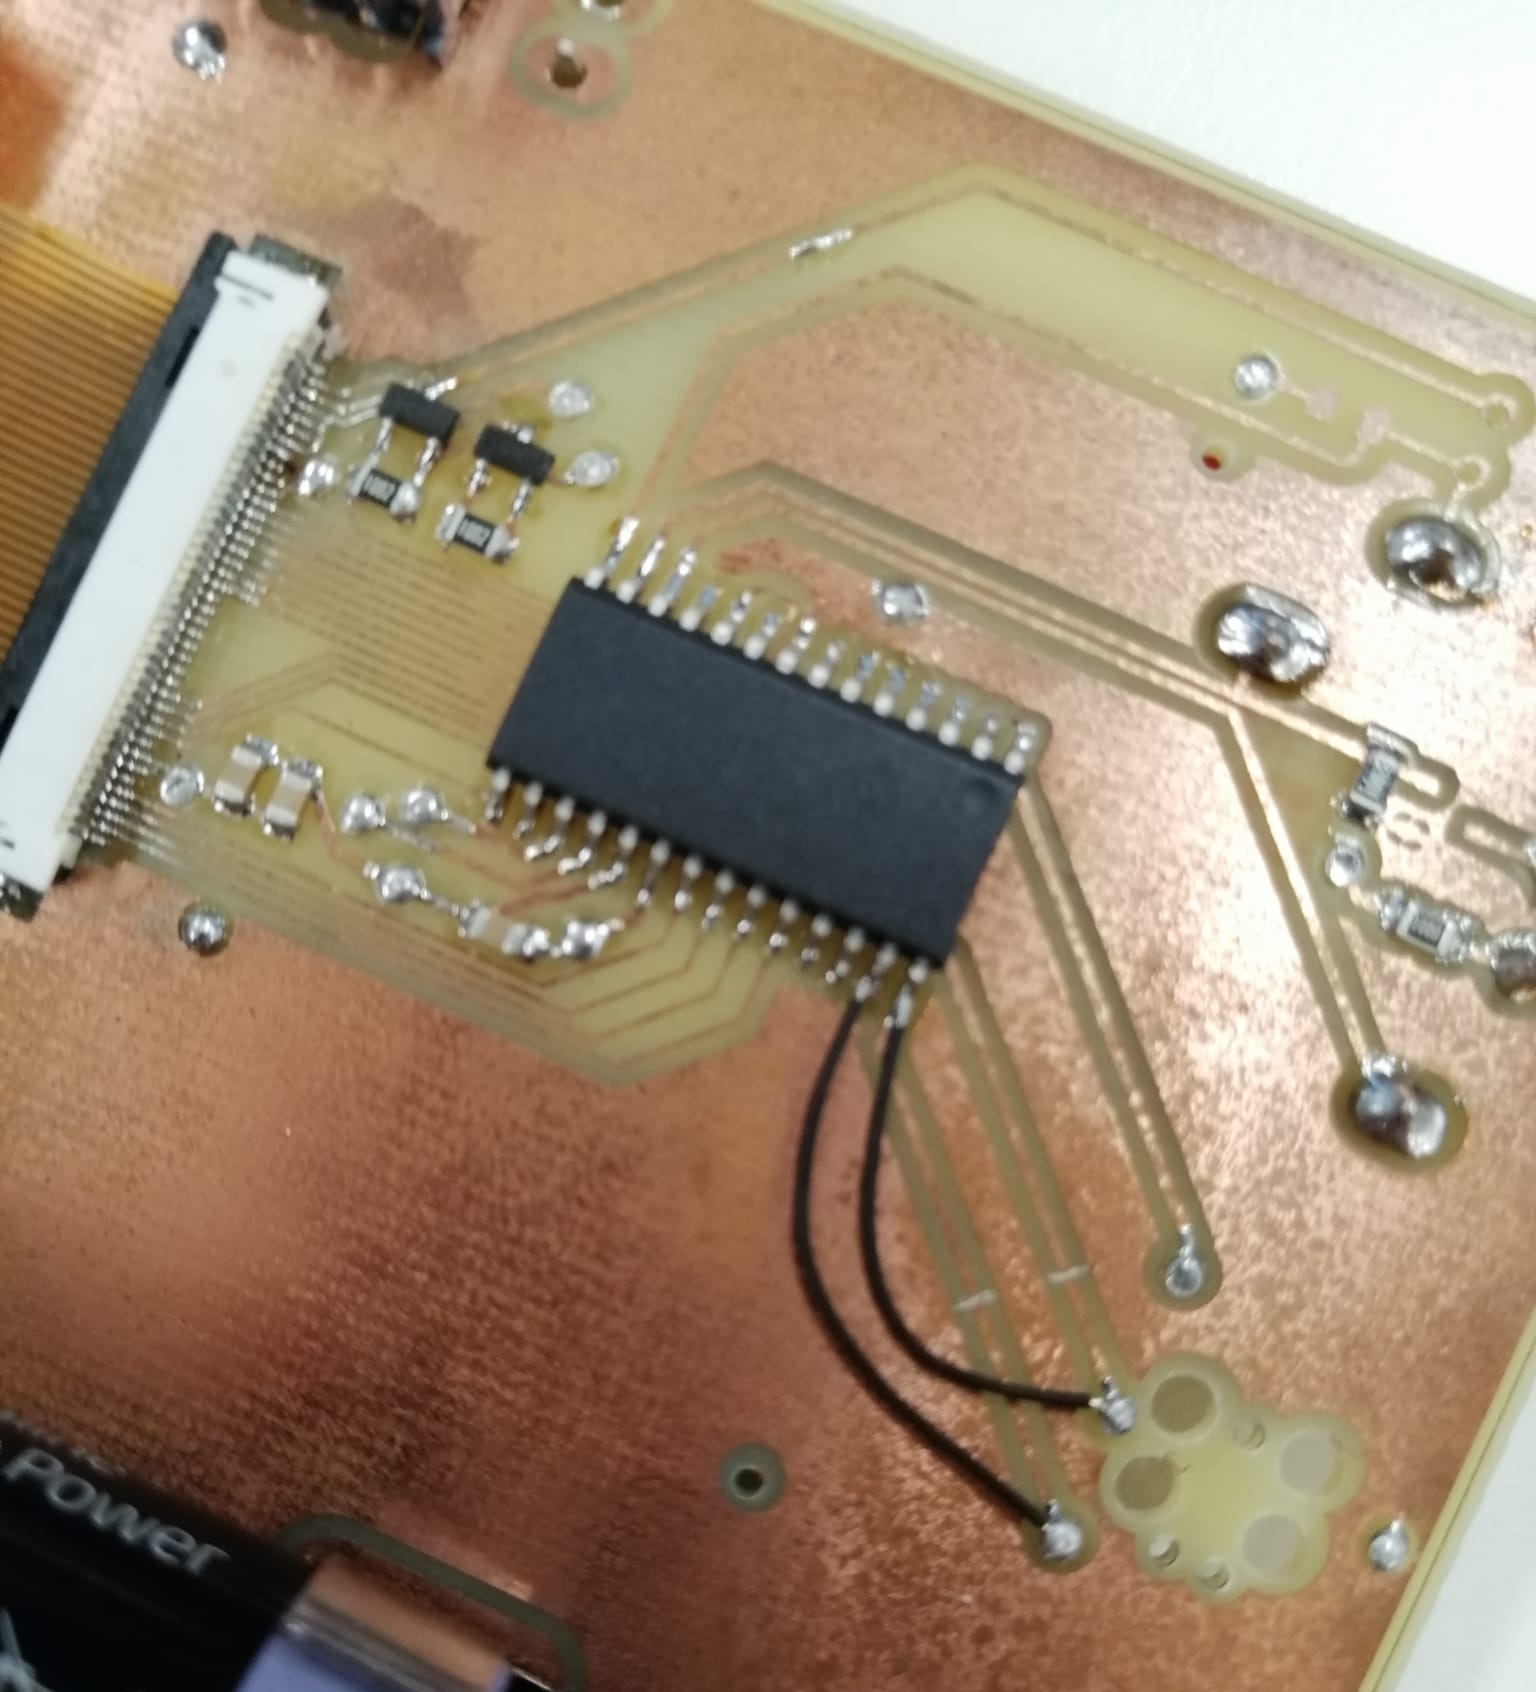
\includegraphics[width=0.5\linewidth]{c_moche}
  \caption{Signaux de programmation PGC et PGD inversés}
  \label{c_moche}
\end{figure}
Par exemple, les signaux PGC et PGD du port de programmation ont été inversé
dans la schématique, résultant en une impossibilité de programmer le processeur.
Cela a été corrigé comme montré dans la figure 3.2

L'ensemble des tests réalisés durant ce projet sont disponibles en Annexe A.
